\documentclass {report}
\usepackage{graphicx}
\usepackage{minted}
\usepackage{titlepic}
%\usepackage[romanian]{babel}
\usepackage{fontspec}

% To draw diagrams.
\usepackage{tikz}
\usepackage{float}
\usetikzlibrary{positioning, arrows.meta}
\usetikzlibrary{fit} % To merge nodes.

%\usepackage[utf8x]{inputec}

\setmainfont{times.ttf}
\definecolor{light_blue}{RGB}{212,235,242}

\title {Relatório de Programação II}

\titlepic{\includegraphics[width=\textwidth]{"game life.png"}}
\author{
  David Marinho\\
  \texttt{54560}
  \and
  Axel Amoroso Carapinha\\
  \texttt{55248}
	\and
	Joana Pimenta\\
	\texttt{51737}
}

\begin {document}
\date{}
\begin{figure}[t]
	\vspace {-2cm}
	\centering
	
\includegraphics[width=0.4\textwidth]{uni_logo.png}
\end{figure}
\maketitle

\section* {Procedimentos}
\begin{enumerate}
  \item Na execução do programa podem ser passados 3 argumentos pela linha de comandos:
		\begin{itemize}
			\item i \(\rightarrow\) O comprimento do prado.
			\item j \(\rightarrow\) A largura do prado. 
			\item starveTime \(\rightarrow\) Número de timesteps a que os coelhos 
					  sobrevivem sem comer qualquer cenoura. Por defeito, se não passados 
						quaisquer argumentos, temos \\i = 100, o j = 100 e starveTime = 5.
		\end{itemize}
	\item Um prado de comprimento i x j é preenchido com objetos do tipo 'Grass'
				e são gerados aleatoriamente outros objetos, objetos de tipo 'Rabbit' e 
				'Carrot'.
	\item A cada timestep é gerado um novo prado respeitando as regras a que
				a geração anterior esteve sujeita.
\end{enumerate}

\section* {Design Patterns}
	Recorremos aos três pilares da Programação Orientada a Objetos, encapsulamento 
	herança e polimorfismo, e criamos quatro classes para representar entidades
	específicas:
	\begin{itemize}
		\item	LifeBeing \(\rightarrow\) Classe mãe e abstrata das classes 'Rabbit',
					'Carrot' e 'Grass'.
		\item	Rabbit \(\rightarrow\) Classe filha que herda 'LifeBeing'. Tem como função 
					organizar todos os dados a respeito dos coelhos.
		\item	Carrot \(\rightarrow\) Classe filha que herda 'LifeBeing'. Organiza 
					toda a estrutura de dados a respeito das cenouras.
		\item	Grass \(\rightarrow\) Classe filha que herda 'LifeBeing' e organiza 
					toda a estrutura de dados a respeitos das ervas.
		\item Grassland \(\rightarrow\) Classe responsável por organizar todos os
					dados a respeito do campo, marioritariamente a posição dos objetos
					no campo e o tempo de longevidade dos mesmos.
		\item Simulation \(\rightarrow\) Classe principal do programa. Responsável
					pela renderização e execução do programa.
	\end{itemize}

	% Draw the Diagram.
	\begin{figure}[h] % See https://tex.stackexchange.com/questions/39017/how-to-influence-the-position-of-float-environments-like-figure-and-table-in-lat for more info.
  %\centering
		\hspace{-2.5cm} % Move whole figure 2.5cm to the left.
		% \vspace{-2.5cm} % Move whole figure 2.5cm up.	
		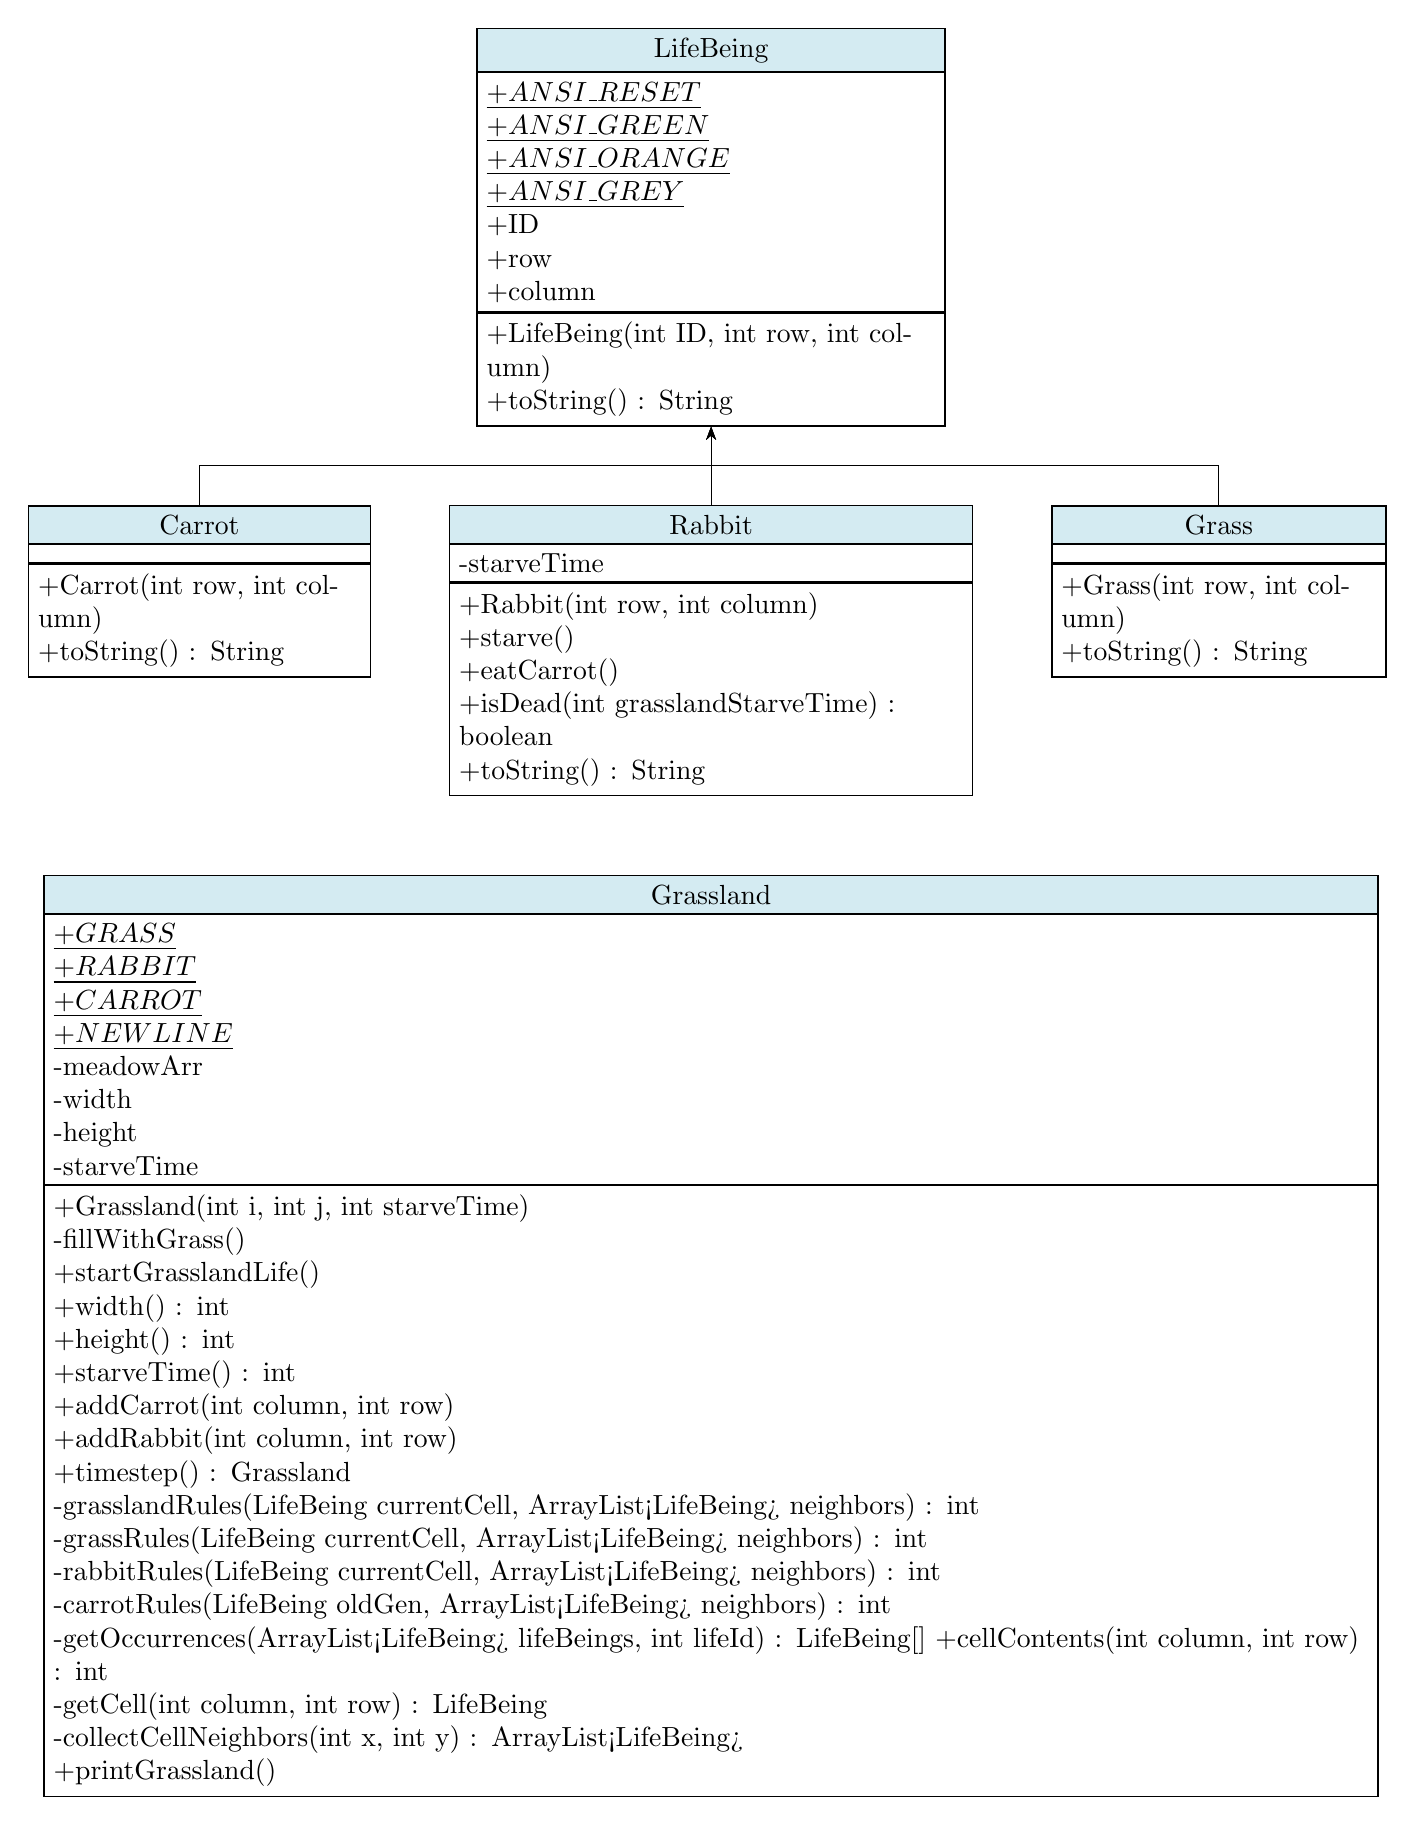
\begin{tikzpicture}[>=Stealth]

    % --- Begin Life Being Node ---
			\node [draw, rectangle, text width=5.7cm, align=center, fill=light_blue] (LifeBeing) {LifeBeing};
		\node [draw, rectangle, text width=5.7cm, below=0.0cm of LifeBeing, align=left] (life_being_attributes) {
			\(\underline{+ANSI\_RESET}\) \\
			\(\underline{+ANSI\_GREEN}\) \\
			\(\underline{+ANSI\_ORANGE}\) \\
			\(\underline{+ANSI\_GREY}\) \\
			+ID \\
			+row \\
			+column \\
    };
		\node [draw, rectangle, text width=5.7cm, below=0.0cm of life_being_attributes, align=left] (life_being_methods) {
			+LifeBeing(int ID, int row, int column) \\
			+toString() : String
    };
    
    % Merge all the nodes so it can turn all this nodes into one.
    \node [draw, fit={(LifeBeing) (life_being_attributes) (life_being_methods)}, inner sep=0pt] (LifeBeingNode) {};
		% --- End Life Being Node ---

		% -- Begin Rabbit Node. ---
    \node [draw, rectangle, below=of LifeBeingNode, text width=6.4cm, align=center, fill=light_blue] (Rabbit) {Rabbit};
		\node [draw, rectangle, text width=6.4cm, below=0.0cm of Rabbit, align=left] (rabbit_attributes) {
			-starveTime
		};
		\node [draw, rectangle, text width=6.4cm, below=0.0cm of rabbit_attributes, align=left] (rabbit_methods) {
			+Rabbit(int row, int column) \\
			+starve() \\
			+eatCarrot() \\
			+isDead(int grasslandStarveTime) : boolean \\
			+toString() : String
		};

    % Merge Rabbit Nodes.
		\node [draw, fit={(Rabbit) (rabbit_attributes) (rabbit_methods)}, inner sep=0pt] (RabbitNode) {};
		% --- End Rabbit Node. ---

		% --- Begin Carrot Node. ---
    \node [draw, rectangle, left=of Rabbit, text width=4.1cm, align=center, fill=light_blue] (Carrot) {Carrot};
		\node [draw, rectangle, text width=4.1cm, below=0.0cm of Carrot, align=left] (carrot_attributes) {};
		\node [draw, rectangle, text width=4.1cm, below=0.0cm of carrot_attributes, align=left] (carrot_methods) {
			+Carrot(int row, int column) \\
			+toString() : String
		};

    % Merge Carrot Nodes.
		\node [draw, fit={(Carrot) (carrot_attributes) (carrot_methods)}, inner sep=0pt] (CarrotNode) {};
		% --- End Carrot Node. ---

		% --- Begin Grass Node. ---
    \node [draw, rectangle, right=of Rabbit, text width=4.0cm, align=center, fill=light_blue] (Grass) {Grass};
		\node [draw, rectangle, text width=4.0cm, below=0.0cm of Grass, align=left] (grass_attributes) {};
		\node [draw, rectangle, text width=4.0cm, below=0.0cm of grass_attributes, align=left] (grass_methods) {
			+Grass(int row, int column) \\
			+toString() : String
    };

    % Merge Grass Nodes.
    \node [draw, fit={(Grass) (grass_attributes) (grass_methods)}, inner sep=0pt] (GrassNode) {};
		% --- End Grass Node. ---

    % Connect the nodes.
    \draw[->] (RabbitNode.north) -- ++(0,0.5) -| (LifeBeingNode.south);
    \draw[->] (CarrotNode.north) -- ++(0,0.5) -| (LifeBeingNode.south);
    \draw[->] (GrassNode.north) -- ++(0,0.5) -| (LifeBeingNode.south);

		% --- Begin Grassland Node ---
    \node [draw, rectangle, text width=16.7cm, below=1.0cm of RabbitNode, align=center, fill=light_blue] (Grassland) {Grassland};
		\node [draw, rectangle, text width=16.7cm, below=0.0cm of Grassland, align=left] (grassland_attributes) {
			\(\underline{+GRASS}\) \\
			\(\underline{+RABBIT}\) \\
			\(\underline{+CARROT}\) \\
			\(\underline{+NEWLINE}\) \\
			-meadowArr \\
			-width \\
			-height \\
			-starveTime \\
    };
		\node [draw, rectangle, text width=16.7cm, below=0.0cm of grassland_attributes, align=left] (grassland_methods) {
			+Grassland(int i, int j, int starveTime) \\
			-fillWithGrass() \\
			+startGrasslandLife() \\
			+width() : int \\
			+height() : int \\
			+starveTime() : int \\
			+addCarrot(int column, int row) \\
			+addRabbit(int column, int row) \\
			+timestep() : Grassland \\
			-grasslandRules(LifeBeing currentCell, ArrayList<LifeBeing> neighbors) : int \\
 			-grassRules(LifeBeing currentCell, ArrayList<LifeBeing> neighbors) : int \\
			-rabbitRules(LifeBeing currentCell, ArrayList<LifeBeing> neighbors) : int \\
			-carrotRules(LifeBeing oldGen, ArrayList<LifeBeing> neighbors) : int \\
			-getOccurrences(ArrayList<LifeBeing> lifeBeings, int lifeId) : LifeBeing[]
			+cellContents(int column, int row) : int \\
		  -getCell(int column, int row) : LifeBeing \\
			-collectCellNeighbors(int x, int y) : ArrayList<LifeBeing> \\ 
			+printGrassland()
    };
    
    % Merge all the nodes so it can turn all this nodes into one.
    \node [draw, fit={(Grassland) (grassland_attributes) (grassland_methods)}, inner sep=0pt] (GrasslandNode) {};
		% --- End Grassland Node ---

  \end{tikzpicture}
  \caption{Diagrama de classes}
\end{figure}

\clearpage % Forces all figures above it in the .tex file to be printed before continuing with the text. This can leave large white spaces. More info in https://tex.stackexchange.com/questions/8625/force-figure-placement-in-text

% Exemplo de insereção de código.
%\begin{minted}[autogobble]{java}
%  public static void main(String[] args) {
%    System.out.println("Hello World!");
%  }
%\end{minted}

\end {document}
